Because standing areas are polygons that consist of nodes, which are connected to each other, they can be viewed as a circular linked list. These have to be saved in the database. The database model is shown in Figure \ref{fig:standing_area_db_model}. All the other tables are left out for simplicity.

\begin{figure}[H]
    \centering
    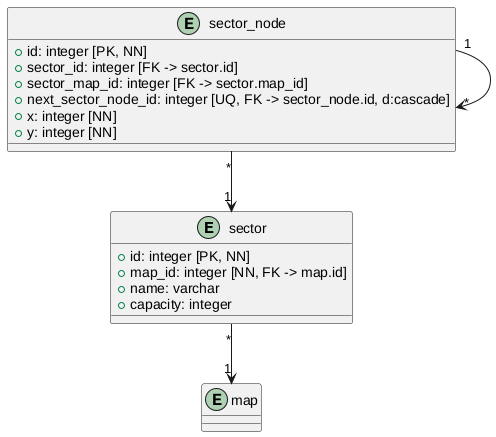
\includegraphics[scale=0.5]{pics/standing-area-db.png}
    \caption{Standing Area Database Model}
    \label{fig:standing_area_db_model}
\end{figure}

The sector\_node entity in the database has a foreign key that references itself. This allows modeling a hierarchy, and in this case, the hierarchy forms a loop. To ensure database integrity, a unique constraint is set on the next\_sector\_node\_id. This makes sure that there is only one sector node that is the successor of a given sector node. When fetching a standing area, two options were considered.

\begin{compactenum}
\item Fetch all sector nodes from a map and build the standing area in the backend.
\item Make a recursive query in the database that fetches all sector nodes of a standing area.
\end{compactenum}

The advantage of the second approach is that only the needed nodes are fetched, and the logic is closer to the database. The main issue is, that SQL queries in Postgres doesn't have  a built-in way to do recursion like Oracle DB has with its \texttt{connect by} clause. The solution for Postgres would have to be implemented with PostgreSQL-specific keywords. A query that fetches all the items in a loop would look as seen in Listing \ref{lst:recursive_query}. 

\newpage

\begin{lstlisting}[language=SQL, caption=Recursive Query, label=lst:recursive_query]
WITH RECURSIVE cte AS (
    -- select first node with level 1
    SELECT *, 1 AS level
    FROM   sector_node
    WHERE  (SELECT id FROM sector_node 
                WHERE map_id = 1 AND sector_id = 1 LIMIT 1
            ) = id

    UNION  ALL
    SELECT  sn.*, c.level + 1 AS level
    FROM cte c
        JOIN sector_node sn ON c.next_sector_node_id = sn.id 
        WHERE (SELECT id FROM sector_node 
                   WHERE map_id = 1 AND sector_id = 1 LIMIT 1
              ) != sn.id
)
SELECT id, x, y
FROM   cte
ORDER  BY level;
\end{lstlisting}

Here the \texttt{WITH RECURSIVE} clause is used to define a recursive query. The query selects the first node and then iterates through the linked list by repeatedly joining the sector\_node table with itself using the next\_sector\_node\_id field. This process continues until all nodes in the loop have been retrieved. The main disadvantage of this approach is that it uses a PostgreSQL-specific keyword. This makes it impossible to seamlessly switch to another database. This is why the first approach was chosen. The standing areas of the map are fetched in the backend and ordered recursively in a way that represents the loop, as shown in Listing \ref{lst:standing_area_backend}.

\begin{lstlisting}[language=Kotlin, caption=Standing Area Backend, label=lst:standing_area_backend]
override fun getSectorNodeBySector(sector: Sector): Set<SectorNode> {
    val startNode = db.getFirstSectorNodeBySector(sector.id!!)
    return startNode.collectSectorNodes(startNode)
}

private fun SectorNode.collectSectorNodes(startNode: SectorNode): Set<SectorNode> {
    return setOf(this) + (
            if (next == startNode) emptySet() 
            else next?.collectSectorNodes(startNode) ?: emptySet()
        )
}
\end{lstlisting}